\chapter{Implementation}
\label{chap:implementation}

In this chapter, we describe how to connect the computer vision algorithms described in Chapter \ref{chap:algorithms} to obtain a program solving the task of 3D reconstruction on a mobile phone. 
The result of this work is an Android application that allows the user to take photos with a camera, browse them and pick a pair of images to reconstruct. 
The reconstructed image is then visualized in 3D using OpenGL~ES.
Recall the properties of the input pair of photos described in Section \ref{prob}.
An example of a suitable pair of images is shown in Figure \ref{fig:input_samples}.

The following are the main obstacles we are faced with when trying to solve this problem: 
\begin{itemize}
\item mobile phones typically have a limited computational power, 
\item they also have limited operational memory, 
\item most importantly, the optical properties of digital cameras included in a typical mobile phone are of mediocre quality at best. 
\end{itemize} 
The last property is particularly troublesome for us, since it implies -- among other problems -- that the captured image is defomed by an unknown non-linear transformation. 
% This is an issue often encountered in professional-grade cameras as well. 
% However, in these cases, this distortion can be efficiently estimated and accounted for since it typically behaves in a constrained manner. 
% For cheap mobile phone cameras, this is not possible and thus we have to keep in mind that 
This implies that the model of projective camera and the epipolar constraints discussed in Section \ref{sec:projective} are only a rough approximation. 
However, this significantly restricts the choice of computer vision algorithms to apply. 
For example, algorithms for the dense reconstruction problem are often heavily dependent on having a precise model of the epipolar constrains in the image pair. 

We solve this issue using a combination of sparse feature matching and the classical optical flow algorithm (both described in Chapter \ref{chap:algorithms}). 
Specifically, we employ the SURF algorithm because it has better computational efficiency compared with the SIFT algorithm.
Sparse feature matching can be successfully performed without any kind of epipolar constraint and therefore the inaccuracy of the camera model is not an issue. 
However, the resulting 3D information is only a sparse 3D point cloud reconstruction of the scene. 
Since this is insufficient for our purposes, we then repeat optical flow calculation on pairs of neighbourhoods of corresponding features. 

% The final section is devoted to technical aspects of the implementation. 

\section{Implementation outline}
\label{sec:impl_outline}
In the this section we describe the way how was the task solved, what algorithms were chosen and how was the application implemented.
At first we find the initial relative position of the pair of the input images.
Then we detect and match SURF keypoints from which is chosen the most robust match to specify the relative position more accurately.
The next step is to detect a larger amount of SURF keypoints. 
The matching process uses the information of the relative position estimated in the previous step and thus obtain significantly larger number of matches.
Finally, we obtain the dense correspondences by detecting even more matches using the optical flow algorithm.
An illustration of the steps of the process is shown in Figure \ref{fig:impl}.

\begin{figure}[H]
\centering

\begin{subfigure}[b]{0.45\textwidth}
\centering
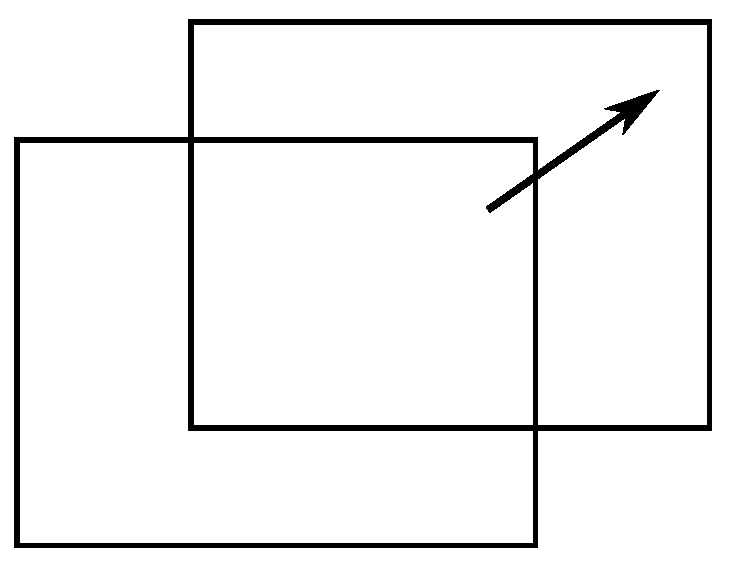
\includegraphics[width=3.8cm]{img/impl0.pdf}
\caption{An overall shift between the photos is computed.} \label{impl0}
\end{subfigure}
\begin{subfigure}[b]{0.45\textwidth}
\centering
\includegraphics[width=6.5cm]{img/impl1.pdf}
\caption{Precise parameters of the translation are identified.} \label{impl1}
\end{subfigure}
\begin{subfigure}[b]{0.45\textwidth}
\centering
\includegraphics[width=6.5cm]{img/impl2.pdf}
\caption{Increasing the density of SURF matches through local matching. Only features inside the bigger rectangle are considered.} \label{impl2}
% Only features inside the bigger rectangle are considered, only features inside the smaller one are accepted as correspondences.
\end{subfigure}
\begin{subfigure}[b]{0.45\textwidth}
\centering
\includegraphics[width=6.5cm]{img/impl3.pdf}
\caption{Optical flow between neighbourhoods of corresponding features is computed to further improve the density of matched pixels.} \label{impl3}
\end{subfigure}

\caption[]{An illustration of the four main stages of our reconstruction pipeline.} 
\label{fig:impl}
\end{figure}

\subsection{The initial relative position}
The first step is illustrated in Figure \ref{impl0}.
Finding the initial relative position of the pair of the images is implemented by using Sum of absolute differences (described in Section \ref{sec:metrics}).
At first, we create an image pyramid, find the overlap of the images in the lowest scale and by upscaling specify the overlapping area more accurately.
In this way the registration runs in approximately two seconds for a pair of the expected input.

\begin{figure}[H]
\centerline{
\includegraphics[width=4.0cm]{img/ema_overlap.png}
\includegraphics[width=4.0cm]{img/ema_buckets.png}}
\caption{Left: The result of the registration where the process of upscaling was stopped when the height of the image was over 200px. Right: The division of an image into square-boxes.}
\label{fig:overlap_and_buckets}
\end{figure}

\subsection{Finding the most robust match}
The next step of the process is detection of features using the SURF detector (it is shown in Figure \ref{impl1}).
The basic approach is to try matching every possible pair of the features between two images.
However, this method is very slow and for our work not acceptable.
We speeded-up the computation by dividing the images into square-boxes of the same size and to each square-box we assign an array of keypoints situated in it.
When finding a match for the feature in the first image, we estimate it's corresponding surrounding area in the second image 
and find the square-boxes which are at least partially situated in it.
From these square-boxes we choose the keypoints lying in the corresponding area and find the best match for the keypoint.
At first we find the most robust match from only the SURF keypoints where the the value of the Hessian reaches the specified value.
Based on this match we estimate the direction of the shift which gives us more accurate relative position of the input pair of images.

\begin{figure}[H]
\centerline{
\includegraphics[width=8cm]{img/ema_direction.png}}
\caption{The most robust match chosen from the keypoints with the Hessian over 4000. According to this match the more accurate relative position of images is estimated.}
\label{fig:robust_match}
\end{figure}

\subsection{Feature matching}
To find larger number of corresponding point and more information about the scene, we match the detected SURF keypoints one more time in the next step (see Figure \ref{impl2}).
Otherwise, our corresponding matches would be too sparse for the 3D reconstruction.
For each keypoint, we calculate the corresponding area of the surroundings in the shape of a rectangle oriented in the direction of the shift.
To avoid mismatches we reject the matches where the matched keypoints differs too much in the orientation or if there is more than one obvious potential points for the match.

%When we know the more accurate relative position of the images, we investigate the keypoints one more time.
%Now we iterate all of them. 
%Each keypoint in the first image we try to match with a keypoint in the estimated corresponding surrounding area in the second image in the shape of oriented rectangle computed based on the more accurate relative image position.
%This oriented rectangle actually consists of two rectangles -- one large and one smaller localised in the middle of the previous one.
%The corresponding keypoint is accepted only if its located in the inner one.
%The size of the larger rectangle is set to 60 $\times$ 120 pixels.
%The inner rectangle after some experiments was set to the 10\% of width and 20\% of height.
%It was shown that it gives better results than only a bit larger window of the the width of 20\% of width and 35\% of height size.
%Matched keypoints which differs too much in the orientation or are not obviously the best match we reject again.
%We can see the comparison in Figure \ref{fig:matching_comparison}.

%Dense correspondence: optical flow::

\subsection{Dense correspondence}
At this point we have relatively robust matches for sparse correspondence. 
For the calculation of the depth information we need to extract more corresponding points.
Assuming the difference of images is limited, we use for this purpose optical flow algorithm. 
For each SURF keypoint in the first image we detect corners or other features acceptable for the tracking algorithm in its 70 $\times$ 70 pixels area.

Calculating the optical flow we get the corresponding points in the second image.
With high probability some of the results will be influenced by noise.
To avoid these mismatches we calculate the variation of the distances between each match.
If the variation is higher than 300 we discard all of the detected optical flow matches.
This stage (illustrated in Figure \ref{impl3}) gives us dense correspondence and enough information to build a 3D reconstruction of the scene.

\section{Graphical visualization}
The result is visualized in OpenGL~ES.
Every keypoint is represented as a triangle in a space with the depth calculated from the correspondence.
The depth is estimated form the distance of the corresponding pair of keypoints. 
The shift is not that remarkable for objects in the background of the image and thus the distance is smaller.
Bigger distance occurs for images situated in the foreground.
We start rendering the model when we obtain the first information about the depth resulted from the SURF matching.
Each time new data from calculation of the dense corresponding points are available, we update the model, so the user can see an animation of the process of execution of our algorithm.


